\documentclass[letterpaper,12pt,dvips]{article}

\usepackage{latexsym}
\usepackage{fancybox}
\usepackage{graphicx}
\usepackage{natbib}
\usepackage{color}
\usepackage{amsmath}
\usepackage{ulem}
\usepackage{float}
\usepackage{here}
\usepackage{multicol}

\pretolerance=10000
\textwidth=6.5in
\textheight=8.9in
\voffset = -0.3in
\topmargin=0.0in
\headheight=0.00in
\hoffset = 0.0in
\headsep=0.00in
\oddsidemargin=0in
\evensidemargin=0in
\parindent=2em
\parskip=1.5ex

\DeclareMathAlphabet{\mathsc}{OT1}{cmr}{m}{sc}
\def\testbx{bx}
\DeclareRobustCommand{\ion}[2]{
\relax\ifmmode
\ifx\testbx\f@series
{\mathbf{#1\,\mathsc{#2}}}\else
{\mathrm{#1\,\mathsc{#2}}}\fi
\else\textup{#1\,{\mdseries\textsc{#2}}}
\fi}

\newenvironment{my_itemize}{
\begin{itemize}
  \setlength{\itemsep}{1pt}
  \setlength{\parskip}{0pt}
  \setlength{\parsep}{0pt}}{\end{itemize}
}

\begin{document}
\noindent {{\bf ID: S000 \hspace{1.3cm} PI: Marie Wingyee Lau \hspace{1.3cm} 
Inst.: Kast\hspace{1.3cm} Req.: 17 nights}}\\[-1cm]
\begin{center}
\bf\Large
A Potentially Transformative Approach to Cluster Cosmology 
\end{center}

\section{Scientific Justification} 

Pinning down the nature of dark energy is one of the most pressing questions in modern physics. Dark energy is thought to be either a cosmological constant with an equation of state $w=P/\rho=-1$ which remains constant at all times, a new type of fluid with an equation of state that varies with time ($w \neq$ constant), or dark energy might indicate a breakdown of Einstein's Theory of General Relativity. It is of critical importance to distinguish between these three scenarios. This can only be accomplished by ambitious and demanding measurements of both the expansion rate of the universe (to track the time evolution of dark energy) together with measurements of the rate at which cosmic structures, such as galaxies and clusters of galaxies, grow with time (the ``growth rate"). The redshift evolution of the abundance of massive clusters is a direct probe the growth of large scale structures.

The Hyper Suprime Cam survey (2014-2019) is a large (1400 deg$^2$), deep (i$\sim$26.5), lensing survey conducted on the Subaru telescope. One of the goals of the HSC survey is to identify galaxy clusters and to constrain the growth of large scale structure in the redshift range where the effects are dark energy are the largest ($z<0.5$). The default plan in HSC, is to identify clusters via the  ``red-sequence" method. In recent years, the quality of optical red-sequence clusters finders has much improved, with the state-of-the-art being the redMaPPer cluster finder \citep[][]{Rykoff:2014,Rozo:2014}. However, as the volume of data increases (imposing correspondingly stricter requirements on systematic errors), three aspects are becoming serious limiting factors:

\begin{enumerate}
\item It is not straightforward to identify the galaxy at the center of the cluster (the ``central galaxy''). This creates mis-centering errors which directly propage into errors on halo masses from weak lensing.
\item Red-sequence cluster finders are prone to projection effects and some ``massive clusters'' are actually two smaller systems projected along the line-of-sight \citep[e.g.,][]{Busch:2017aa}. Conversely, red-sequence cluster finders also sometimes accidentally break up massive clusters into two smaller systems (``fragmentation''). 
\item The solution to 1) and 2) is to forward model the cluster finding process by running red-sequence cluster finders on mock observations. However, building mock catalogs that are reliable enough to completely forward model this process is a long standing issue in this field to which there is no immediate solution at hand.
\end{enumerate}


With these challenges in mind, our group has been using HSC data to explore some exciting and potentially transformative new ideas about optical cluster finding. The basic idea, while exceedingly simple, appears to be performing amazingly well. Our approach is based on the idea that galaxies that live at the very centers of clusters (BCGs; Brightest Cluster Galaxies) have extended light profiles which distinguish them from other galaxies \citep[][Huang et al. in prep]{Huang:2017a}. With deep enough data, we are finding that BCGs can be identified directly based their extended light profiles and their luminosities. Why has this method not been used previously? Mainly because of a prevailing consensus that the luminosities of central galaxies do not correlate with halo mass as well as ``richness'' estimators such as the redMaPPer $\lambda$ parameter\footnote{The logarithmic scatter in halo mass at fixed $\lambda$ is thought to be lower than the scatter in halo mass at fixed galaxy mass ($\sigma_{Mhalo|\lambda}=0.16$ dex < $\sigma_{Mhalo|M*}=0.25$ dex)}. With more in-depth investigation, however, we are finding that these ideas stem from the use of shallow imaging data (such as SDSS) and poorly estimated luminosities. Instead, with deeper data, and using more carefully extracted luminosities \citep[][]{Huang:2017a}, our weak lensing test are showing that the luminosities of central galaxies trace halos as well (and possibly even better) than $\lambda$!

Our new approach has advantages over red-sequence based methods for all three key points 1), 2), and 3). Our method identifies BCGs directly via their extended light profiles and projection effects should be minimal. Furthermore, the simplicity of this method imposes less stringent requirements on mock catalogs. Mocks for this cluster finder would only need to model the connection between massive central galaxies and their halos (a more simple task than modeling the full red-sequence population).

The massive galaxy catalog that we intend to use to apply this method to HSC is comprised of super massive galaxies ($\log(M_*)>11.5$) at $z<0.5$. The majority of galaxies in our sample have spectrosocpic redshifts from either the GAMA survey, or the BOSS survey. However, there are still a small number of galaxies i our sample for which we are lacking redshifts. \textbf{The goal of this proposal is to aquire spectrosocpic redshift for galaxies in our sample which currenlty only have a photoz}. This is critical to our science because it will enable us to confirm the redshifts of the clusters, to disentangle projection effects, and also to remove a small number of satellite galaxies. The number density of galaxies for which we do not already have a redshift is very low (less than one per square degree). Therefore, aquire spectrosocpic redshifts cannot benefit from any multiplexing advantages and so our targets are well suited for single slit spectroscopy with KAST. The spectroscopically complete sample that we will compile will be similar to the DESI Bright Galaxy Survey (BGS). Thus, our sample will also of tremendous values for the preparation of the DESI spectrocopic survey.


Currently, the total number of galaxies in the cluster catalogs with spectroscopic redshifts is 
XX. With Kast observations, we will eventually add 61 galaxies in three different GAMA fields that 
currently only have photometric redshifts in the catalogs. We cut this target sample at stellar 
mass $M_*>10^{11.5}\,{\rm M}_\odot$, with nearby pair at $<1$\,Mpc, and at 
$0.25<z_{\rm phot}<0.55$. We make a generous cut on photometric redshifts to ensure that all 
$0.3 < z < 0.5$ objects are covered. 

Our major analysis work is to fit the Kast spectra with independent component stellar templates 
using pPXF (Cappellari \& Emsellem 2004), with emphasis on the 4000\,\AA\ break. We were granted 
director's discretionary time in 2017 July for a trial Kast run. We observed four galaxies that 
have spectroscopic redshifts already determined in SDSS, to determine the signal-to-noise required 
for deriving reliable spectroscopic redshifts using Kast, and the brightness limit of the 
galaxies. We observed four galaxies of SDSS magnitude $r=20.0$, $r=19.3$, $r=18.4$, and $r=18.8$, 
each with exposure time $3600\textrm{---}7200$\,s. We performed preliminary data reduction using 
PYPIT. Figure 1 shows the Kast spectra smoothed for clarity, the SDSS spectra, and the models. 
While proper fluxing and cosmic ray rejection are still in progress, we demonstrated that 
signal-to-noise of $\approx5$ is sufficient for measuring redshift with precision of 
$XX\,{\rm km\,s^{-1}}$. In turn, this implies our program is feasible for galaxies with $r<20.0$. 

\clearpage

\noindent{{\bf\large References}}
\begin{my_itemize}
\item[] Last name First name, year, journal
\end{my_itemize}

\begin{figure}[hbt]
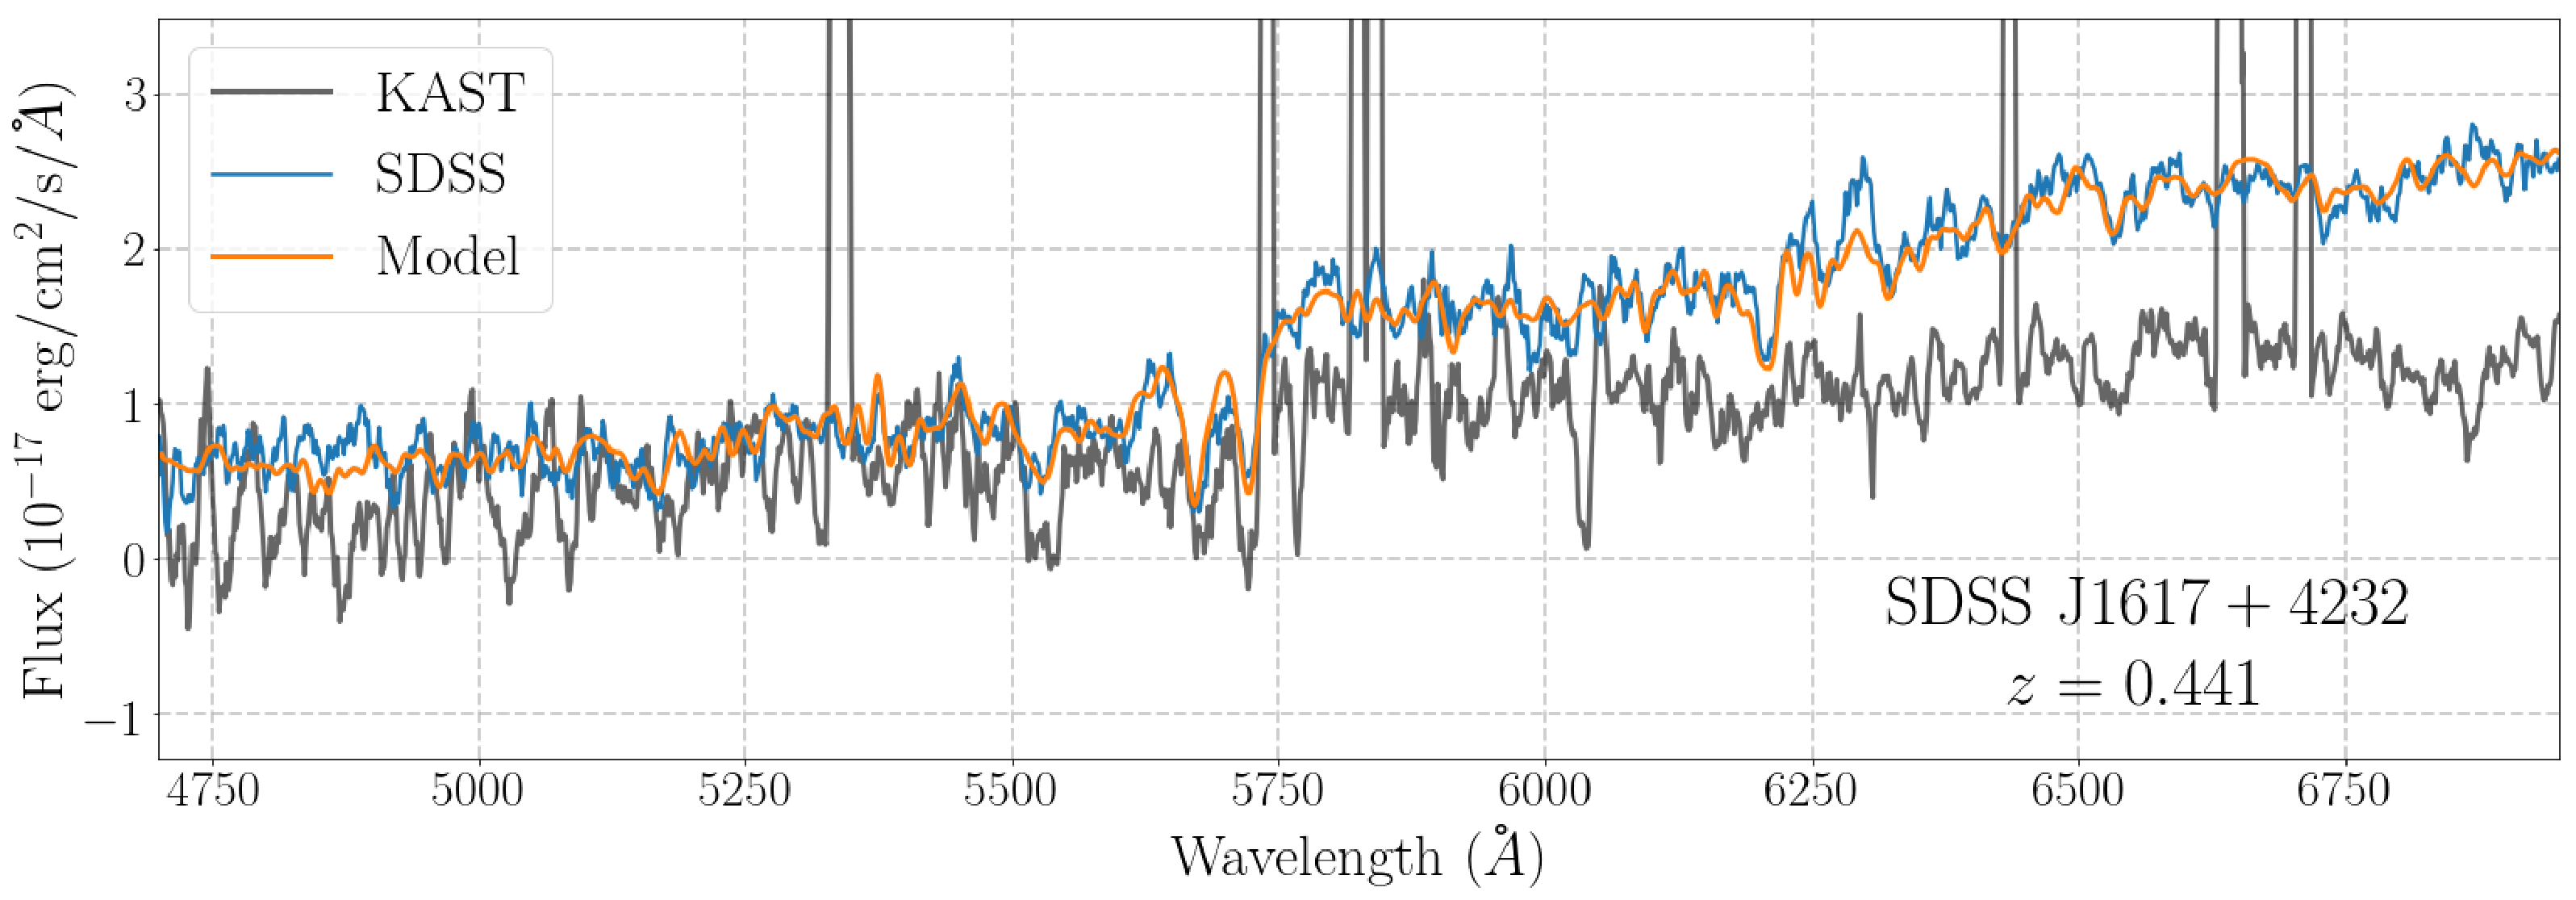
\includegraphics[width=4.0in]{J1617.eps}
\includegraphics[width=4.0in]{J1620.eps}
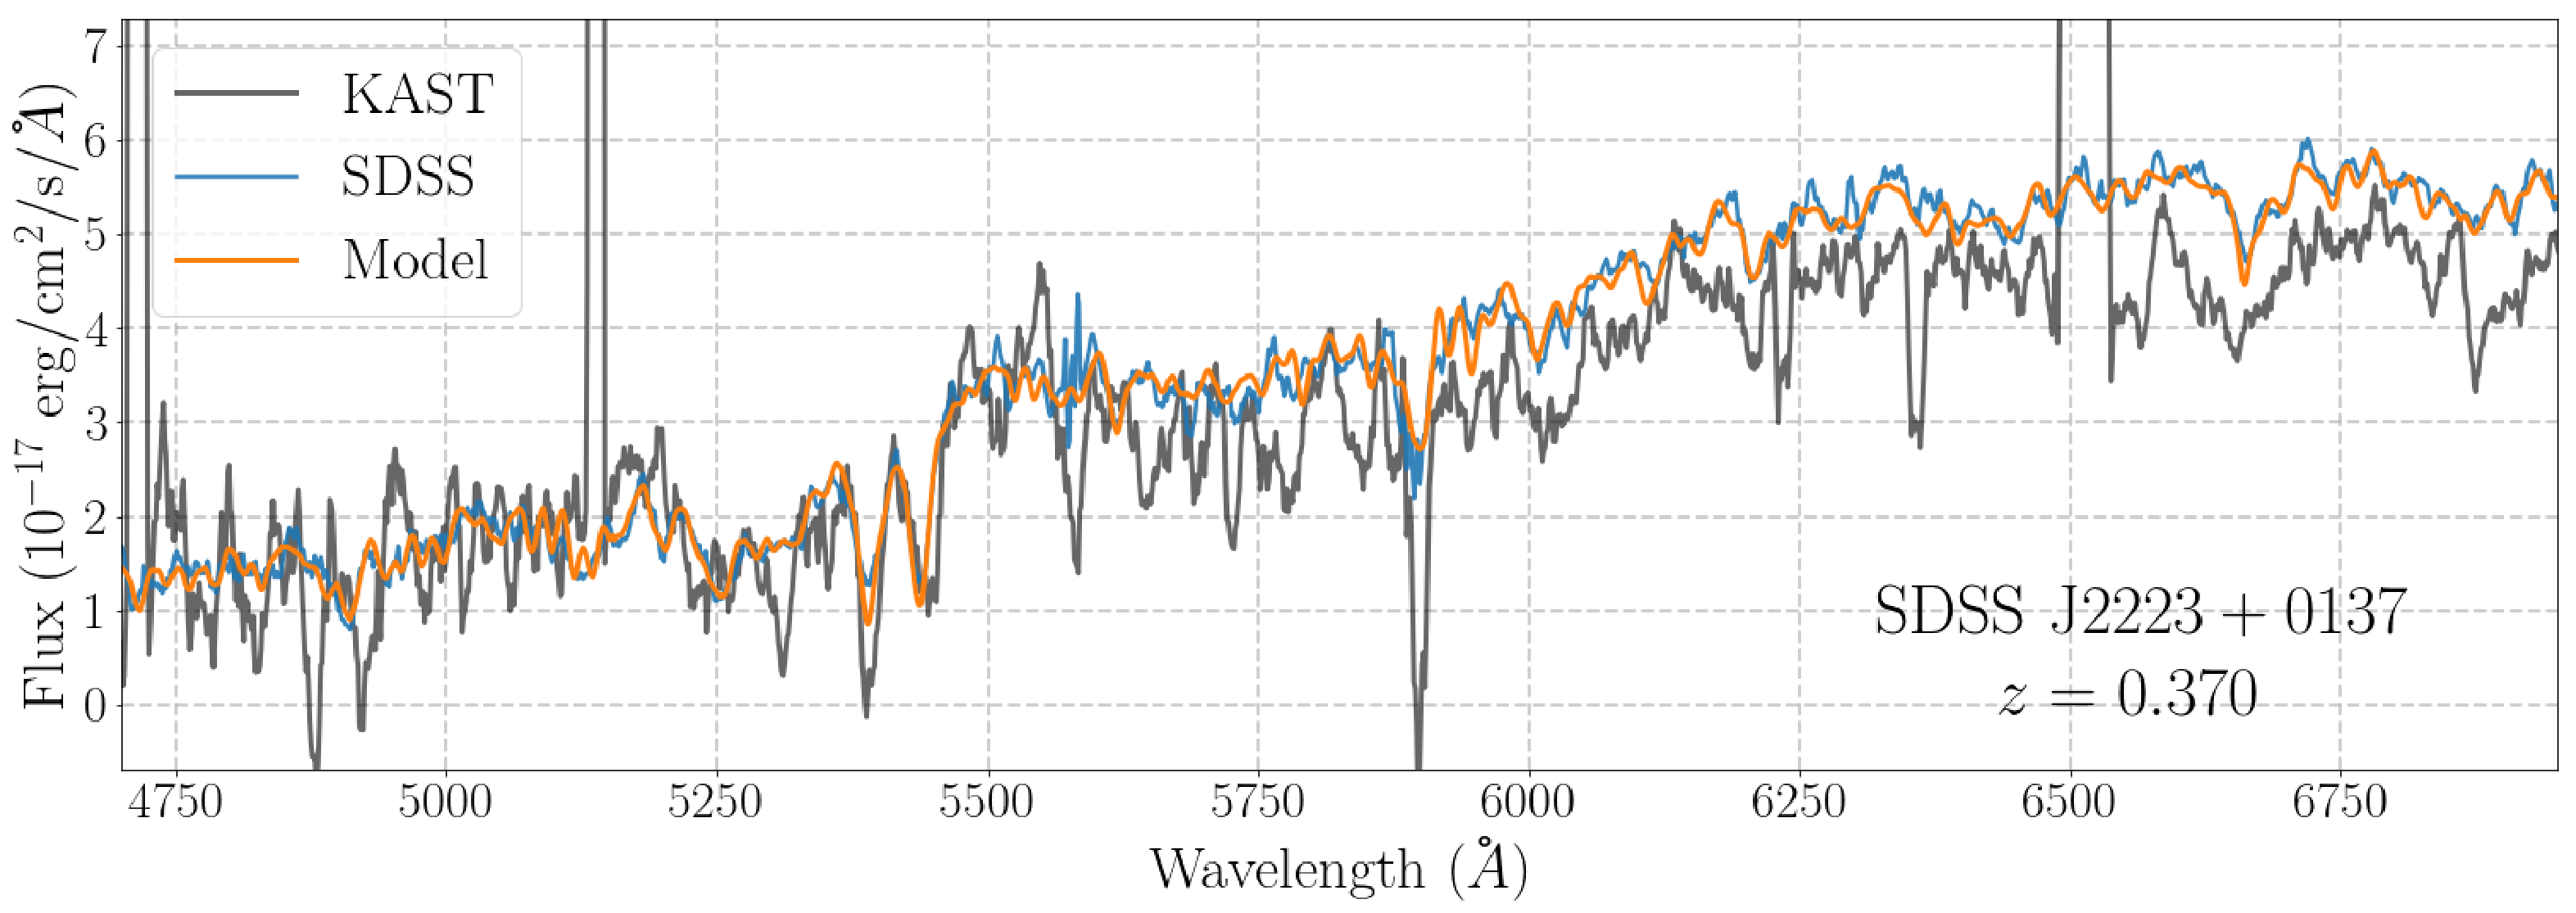
\includegraphics[width=4.0in]{J2223.eps}
\includegraphics[width=4.0in]{J2240.eps}
\caption{
Preliminarily reduced and smoothed Kast spectra of four massive galaxies taken in our trial run in 
2017 July, SDSS spectra of the same galaxies, and the galaxy stellar continuum models generated by 
pPXF. With signal-to-noise of $\approx5$, redshift can be determined with a precision of 
$XX\,{\rm km\,s^{-1}}$.}
\end{figure}

\begin{figure}[hbt]
\includegraphics[width=4.0in]{hsc_fields_2018_02.eps}
\includegraphics[width=4.0in]{hsc_fields_2018_06.eps}
\caption{(Top) visibility curves of the GAMA-A, GAMA-B, and GAMA-C fields on 2018 February 1. 
(Bottom) visibility curves on 2018 June 1.}
\end{figure}

\clearpage

\section{Targets and Exposures}

We will use the Shane 3m telescope and the Kast spectrograph to observe a sample of 39 early-type 
galaxies that currently have photometric redshifts, in three different fields covered by GAMA, 
named GAMA-A, GAMA-B, and GAMA-C. Given the faintness of our targets, dark time is preferred.  

The SDSS $r$-band magnitudes for our targets range between XX and XX. Our science goal will 
require $\sim7200$\,s of exposure to obtain sufficient signal-to-noise. These long exposures will 
be broken into 1800\,s exposures as a compromise between CCD read noise and cosmic ray 
accumulation. 
With overhead we expect we can observe $\approx3$ targets per night. To observe a total of 39 
targets, 13 nights are required at minimum. If available, this program could use an additional 4 
nights to account for unfavorable observing conditions and possibly observe additional galaxies in 
the whole Hyper Suprime-Cam footprint. Figure 2 shows the visibility curves of the four fields to 
be observed on 2018 February 1 and 2018 June 1. Because of the low declination, our targets are 
only observable in a relatively narrow range of time in a semester. We request time allocation in 
March and April when more of our targets are within the telescope pointing limit. 

We will setup to resolve the 4000~\AA\ break and other major spectroscopic features such as 
the Ca II H and K lines, while simultaneously cover a sufficiently broad wavelength range for full 
SED fitting (Figure 1). As a compromise of the above two requirements, we will use the 600/5000 
grating on the red side. 

Table 1 lists all the galaxies in the targeted fields. We will observe additional targets in the 
Hyper Suprime-Cam footprint if we run out of targets. 

In poor observing conditions we will increase exposure time and give preference to bright targets. 

\begin{table}
\caption{List of targets.}
\begin{tabular}{lllllll}
\hline
Name & RA (J2000) & Dec (J2000) & SDSS $r$-mag & photo-$z$ & Exposure \\
JXXXX+XXXX & XX:XX:XX.XX & XX:XX:XX.X & XX.X & X.X & XXXX s & \\
\hline
\end{tabular}
\end{table}

\section{Supplementary Observations Required from other Observatories}

Our full cluster catalogs include spectroscopic redshift catalogs from the GAMA team. 

\section{Technical Remarks}

We have none. 

\subsection{Status of Previously Approved 3-m Programs}

This program obtained director's discretionary time of one night in 2017A. 

PI Lau is a graduate student at UCSC, who has been awarded a total of 22 nights in 2015A, 2016A, 
and 2017A for the program Late-time Optical Spectral Signatures of Tidal Disruption Candidates. 
The observing program is completed and the path to publication is active. 

Co-I Leauthaud and co-I Huang have extensive experience with optical spectroscopy and are experts 
in assive galaxies. 

Co-I Greg Sallaberry is an aspiring undergraduate researcher at UCSC, who will lead the observing 
and data reduction effort. 

\end{document}

